% !TEX TS-program = pdflatex
% !TEX encoding = UTF-8 Unicode

% This is a simple template for a LaTeX document using the "article" class.
% See "book", "report", "letter" for other types of document.

\documentclass[11pt]{article} % use larger type; default would be 10pt

\usepackage[utf8]{inputenc} % set input encoding (not needed with XeLaTeX)
\usepackage{graphicx}
\usepackage{listings}
\usepackage{xcolor}

%%% Examples of Article customizations
% These packages are optional, depending whether you want the features they provide.
% See the LaTeX Companion or other references for full information.

%%% PAGE DIMENSIONS
\usepackage{geometry} % to change the page dimensions
\geometry{a4paper} % or letterpaper (US) or a5paper or....
% \geometry{margin=2in} % for example, change the margins to 2 inches all round
% \geometry{landscape} % set up the page for landscape
%   read geometry.pdf for detailed page layout information

\usepackage{graphicx} % support the \includegraphics command and options

% \usepackage[parfill]{parskip} % Activate to begin paragraphs with an empty line rather than an indent

%%% PACKAGES
\usepackage{booktabs} % for much better looking tables
\usepackage{array} % for better arrays (eg matrices) in maths
\usepackage{paralist} % very flexible & customisable lists (eg. enumerate/itemize, etc.)
\usepackage{verbatim} % adds environment for commenting out blocks of text & for better verbatim
\usepackage{subfig} % make it possible to include more than one captioned figure/table in a single float
% These packages are all incorporated in the memoir class to one degree or another...

%%% HEADERS & FOOTERS
\usepackage{fancyhdr} % This should be set AFTER setting up the page geometry
\pagestyle{fancy} % options: empty , plain , fancy
\renewcommand{\headrulewidth}{0pt} % customise the layout...
\lhead{}\chead{}\rhead{}
\lfoot{}\cfoot{\thepage}\rfoot{}

%%% SECTION TITLE APPEARANCE
\usepackage{sectsty}
\allsectionsfont{\sffamily\mdseries\upshape} % (See the fntguide.pdf for font help)
% (This matches ConTeXt defaults)

%%% ToC (table of contents) APPEARANCE
\usepackage[nottoc,notlof,notlot]{tocbibind} % Put the bibliography in the ToC
\usepackage[titles,subfigure]{tocloft} % Alter the style of the Table of Contents
\renewcommand{\cftsecfont}{\rmfamily\mdseries\upshape}
\renewcommand{\cftsecpagefont}{\rmfamily\mdseries\upshape} % No bold!

%%% END Article customizations

\title{Project Report}
\author{Group 18: Chengzhen Wu, Huiqi Mao, Ruofan Zhou}
%\date{} % Activate to display a given date or no date (if empty),
         % otherwise the current date is printed 

\begin{document}
\maketitle

\section{ER model}
After reading the feedback of diverable1, we modified our ER model as below:\\ \\
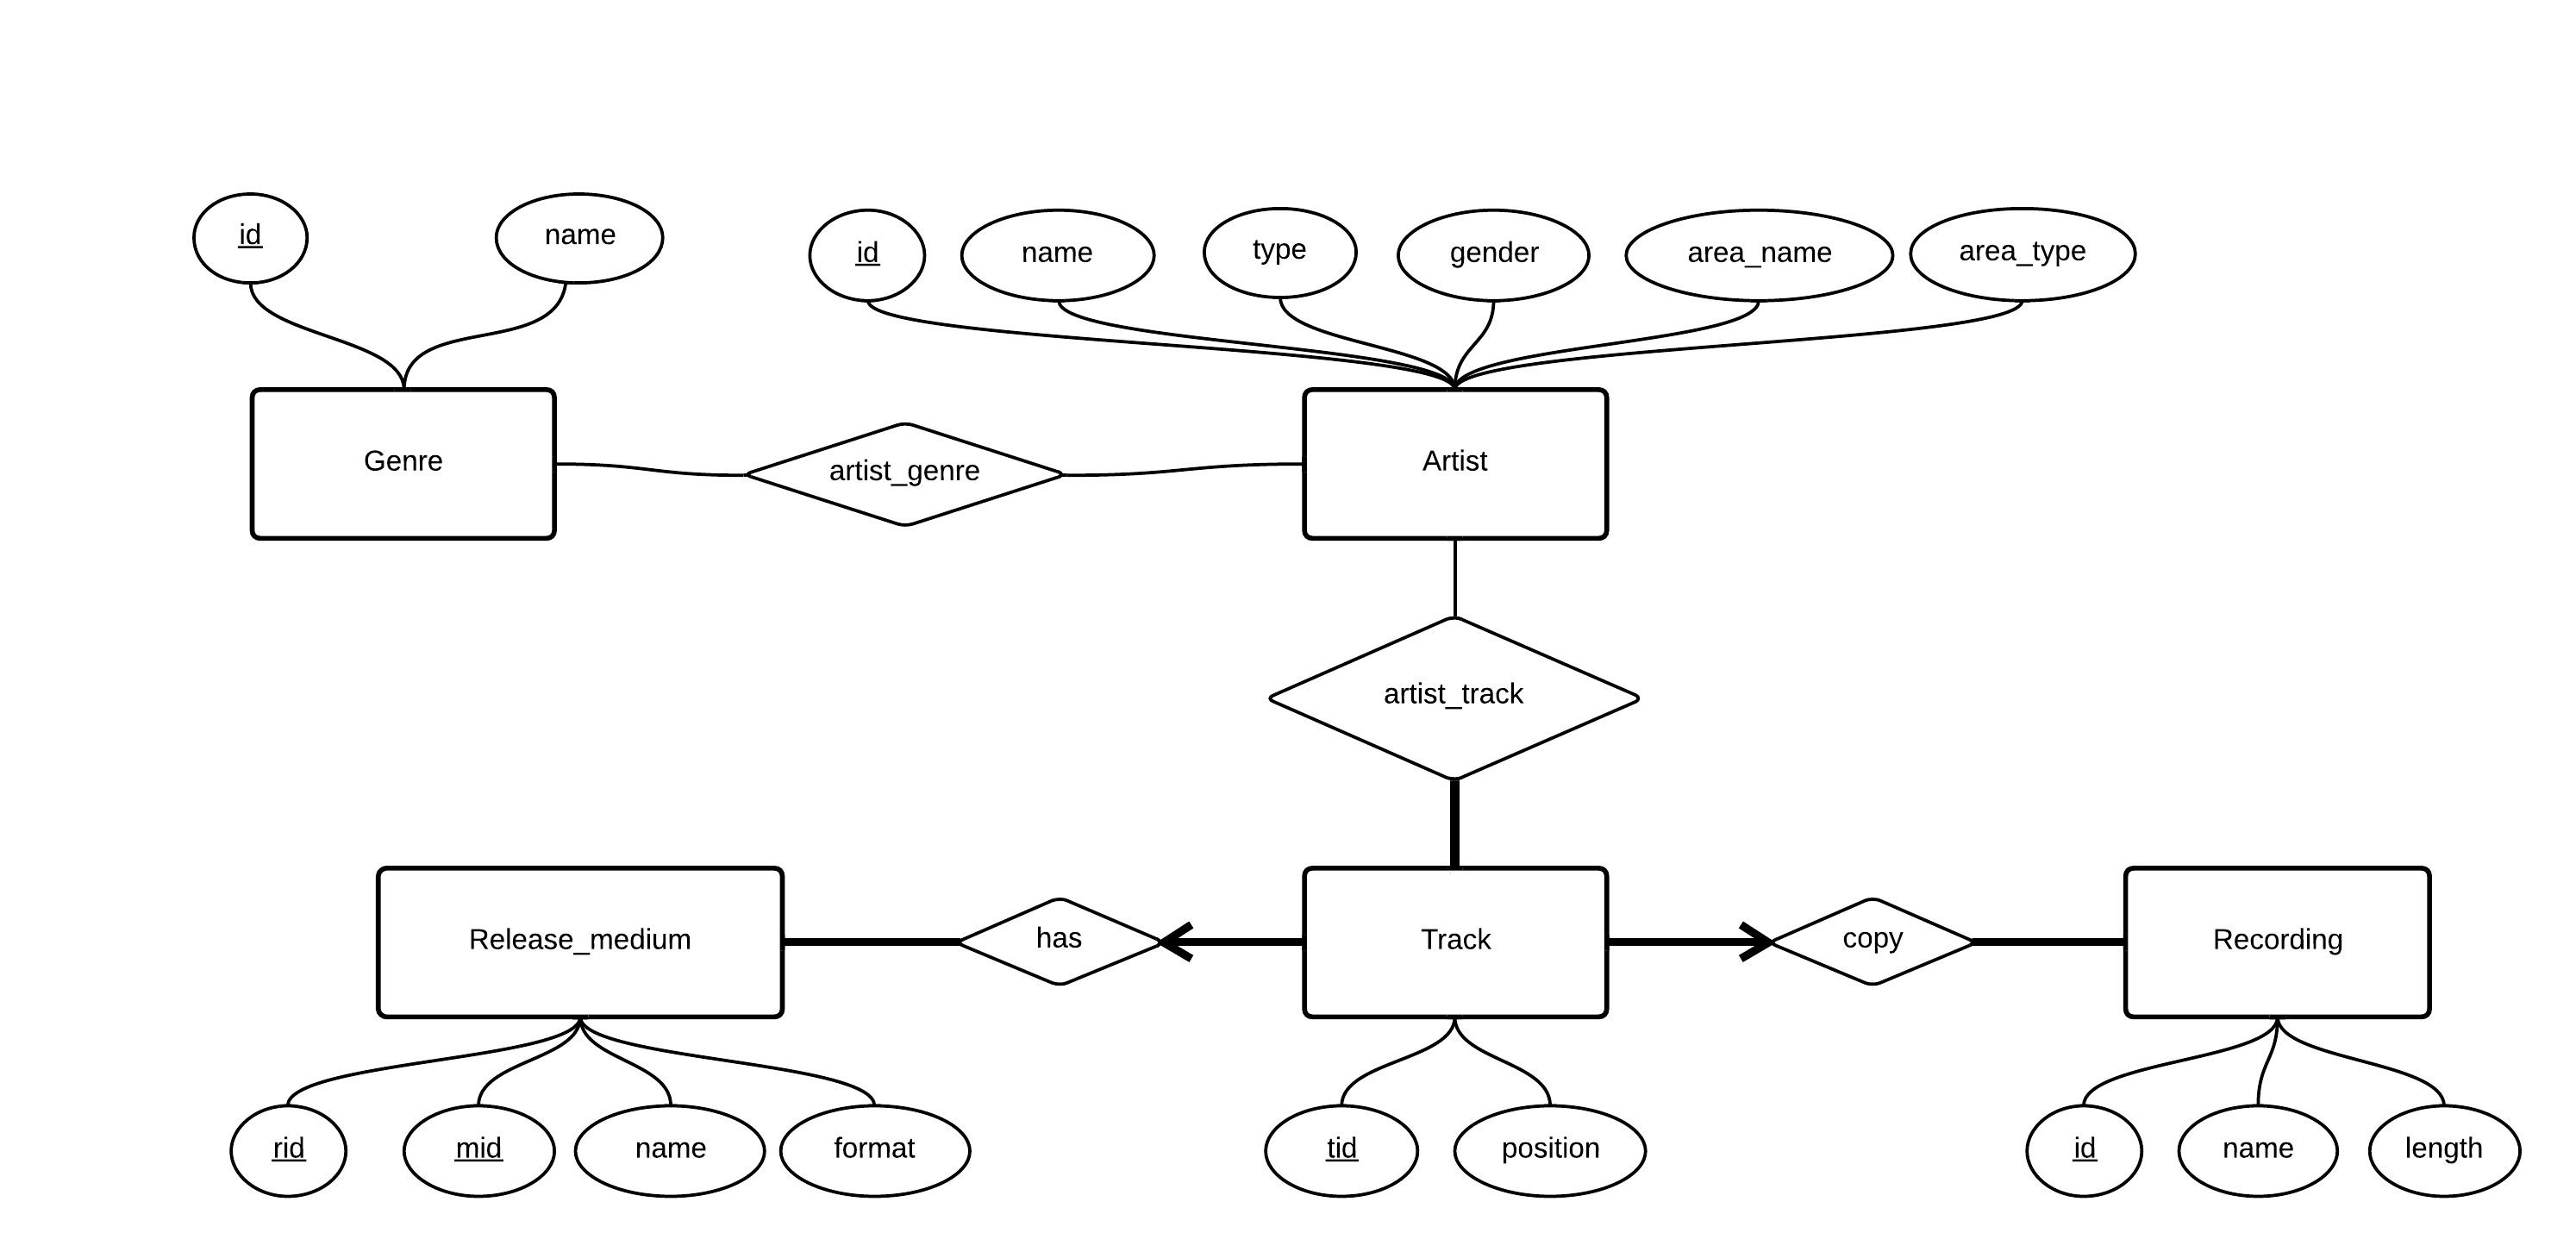
\includegraphics[width=14cm]{ERmodel}\\ \\
In the given project data, we firstly recognize 'area', 'artist' and 'genre' each as three individual entities. Each artist is from at most one area, so it's a many-to-one relation. Several artists can belong to different genres and one genre can contain several artists. So the relation between 'artist' and 'genre' is many-to-many.\\ \\
Secondly, we think about the relationship among 'release', 'recording', track' and 'medium'. We imagine a scene to describe these relations. The csv file of 'release' contains the names of releases. They could be stored in the mediums, such as CD, 12” Vinyl and so on. What's more, one release could have several CDs to contain many tracks, or in different medium (I'm not sure about this, but possible). So the relation between 'release' and 'medium' is one-to-many. Next, each track in different mediums must correspond to one recording. So the relation between 'track' and 'recording' is many-to-one. Each 'track' must be in one of 'medium's. So the relation is many-to-one.\\ \\
Finally, we merge one-to-may relations. 'release' and 'medium' are merged into 'Release\_medium'.  'area' can be merged into 'artist' as attributes. The 'has' relation between 'Release\_medium' and 'track' is merged into 'track' using 'mid' as foreign key. So is the 'copy' relation between 'recording' and 'track' using 'id' of recording as foreign key.\\ \\
Additionally, we ignore the 'count' in 'genre', which could be created as view in the database.\\ \\

\tiny{
\section{SQL based on ER model}
\begin{lstlisting}[language=SQL, keywordstyle=\color{blue!70},
commentstyle=\color{red!50!green!50!blue!50},
rulesepcolor=\color{red!20!green!20!blue!20},
frame=shadowbox]
--ENTITY Genre
--we don't need gcount in genre
CREATE TABLE  Genre (
  GID INTEGER,
  Gname VARCHAR(100),
  PRIMARY KEY (GID)
  );

--ENTITY Artist
CREATE TABLE  Artist (
  AID INTEGER,
  Aname VARCHAR(100),
  Atype CHAR(6),
  gender CHAR(6),
  area_name VARCHAR(60),
  area_type CHAR(15)
  PRIMARY KEY (AID)
  );
  
--ENTITY Recording
CREATE TABLE  recording (
  RID INTEGER,
  Rname VARCHAR(100),
  Rlength INTEGER,
  PRIMARY KEY (RID)
  );

--ENTITY RelaseMedium
CREATE TABLE  ReleaseMedium (
  MID INTEGER,
  RID INTEGER,
  name VARCHAR(400),
  format CHAR(45),
  PRIMARY KEY (RID,MID)
  );

--ENTITY Track
CREATE TABLE  Track (
  TID INTEGER,
  position INTEGER,
  MID INTEGER NOT NULL,
  RID INTEGER NOT NULL,
  REID INTEGER NOT NULL,
  PRIMARY KEY (TID),
  FOREIGN KEY (RID,MID) REFERENCES ReleaseMediuma ON DELETE NO ACTION,
  FOREIGN KEY (REID) REFERENCES Recording ON DELETE NO ACTION
  );
    
--RELATIONSHIP artist_genre
CREATE TABLE artist_genre (
  AID INTEGER NOT NULL,
  GID INTEGER NOT NULL,
  PRIMARY KEY (AID, GID),
  FOREIGN KEY (AID) REFERENCES Artist ON DELETE NO ACTION ,
  FOREIGN KEY (GID) REFERENCES Genre ON DELETE NO ACTION
  );
    
--RELATIONSHIP artist_track
CREATE TABLE artist_track(
  AID INTEGER NOT NULL,
  TID INTEGER NOT NULL,
  PRIMARY KEY (AID, TID),
  FOREIGN KEY (AID) REFERENCES Artist ON DELETE NO ACTION ,
  FOREIGN KEY (TID) REFERENCES Track ON DELETE NO ACTION 
  );
\end{lstlisting}}

\section{Alternative based on Real Data}
\normalsize{
When importing the real data, we find several problems. So we decide to change the schema in order to import as much data as possible. \\ \\
In our ER model, we merged the 'area' and 'artist'. However, since the data is not incomplete, a few AreaIDs in 'artist' don't appear in 'area', such as 'AreaID=241'. So we use an 'area' entity instead. And the foreign key in 'artist' is disabled. Other foreign key constraints, except in 'medium', are also disabled to make it easy to import data. Additionally, in the original file of 'artist.csv', we change '\\N' to '0', which is null in the 'area' table.\\ \\
Another problem with the data is deplicate, since the data in artist\_track has duplicate, we set the foreign-key disabled in the table artist\_track.\\ \\
We separate the release\_medium table into 'release' and 'medium', considering the limited space. Because the name of release could be very long. Duplication could  cause a waste of memory. But the foreign key in 'medium' is still retained, because it works.\\ \\
In the 'genre' entity, 'count' is remained for further possible queries(We find that 'count' from real data is not really the count we caculate).\\ \\}
\section{Alternative SQL}
\tiny{
\begin{lstlisting}[language=SQL, keywordstyle=\color{blue!70},
commentstyle=\color{red!50!green!50!blue!50},
rulesepcolor=\color{red!20!green!20!blue!20},
frame=shadowbox]
CREATE TABLE  Init_Genre (
  GID VARCHAR(20),
  Gname VARCHAR(300),
  count Integer,
  PRIMARY KEY (GID)
  );

create table Init_Area(
  AreaID VARCHAR(20),
  AreaName VARCHAR(150),
  Area_type VARCHAR(15),
  PRIMARY KEY (AreaID)
  );
  
CREATE TABLE  Init_Artist (
  AID VARCHAR(20),
  Aname VARCHAR(200),
  Atype CHAR(10),
  gender CHAR(6),
  --area_name VARCHAR(100),
  --area_type CHAR(15),
  AreaID VARCHAR(20),
  PRIMARY KEY (AID),
  foreign key (AreaID) references Init_area(AreaID)
  );
  
CREATE TABLE Init_Recording (
  RID VARCHAR(20),
  Rname VARCHAR(2000),
  Rlength VARCHAR(20),
  PRIMARY KEY (RID)
  );


CREATE TABLE Init_Release (
  RID VARCHAR(20),
  name VARCHAR(1000),
  PRIMARY KEY (RID)
  );

CREATE TABLE Init_Medium (
  MID VARCHAR(20),
  RID VARCHAR(20),
  format CHAR(45),
  PRIMARY KEY (MID),
  FOREIGN KEY (RID) REFERENCES Init_Release(RID)
  );


CREATE TABLE  Init_Track (
  TID VARCHAR(20),
  REID VARCHAR(20) NOT NULL,
  MID VARCHAR(20) NOT NULL,
  position INTEGER,
  PRIMARY KEY (TID),
  FOREIGN KEY (MID) REFERENCES Init_Medium(MID),
  FOREIGN KEY (REID) REFERENCES Init_Recording(RID)
  );

CREATE TABLE Init_artist_genre (
  AID VARCHAR(20) NOT NULL,
  GID VARCHAR(20) NOT NULL,
  PRIMARY KEY (AID, GID),
  FOREIGN KEY (AID) REFERENCES Init_Artist(AID) ON DELETE CASCADE,
  FOREIGN KEY (GID) REFERENCES Init_Genre(GID) ON DELETE CASCADE
  );

CREATE TABLE Init_artist_track(
  AID VARCHAR(20) NOT NULL,
  TID VARCHAR(20) NOT NULL,
  PRIMARY KEY (AID, TID),
  FOREIGN KEY (AID) REFERENCES Init_Artist(AID), --these foreign keys are disabled for data duplicate
  FOREIGN KEY (TID) REFERENCES Init_Track(TID)
  );
\end{lstlisting}}

\normalsize{
\section{Queries}
We finished the queries based on our model: \\ \\
A
\begin{lstlisting}[language=SQL, keywordstyle=\color{blue!70},
commentstyle=\color{red!50!green!50!blue!50},
rulesepcolor=\color{red!20!green!20!blue!20},
frame=shadowbox]
select artist.ANAME from init_area area, init_artist artist
			where area.areaname='Switzerland';
\end{lstlisting}
B
\begin{lstlisting}[language=SQL, keywordstyle=\color{blue!70},
commentstyle=\color{red!50!green!50!blue!50},
rulesepcolor=\color{red!20!green!20!blue!20},
frame=shadowbox]
select area.areaname
from INIT_AREA area
where area.AREAID in (select art.areaid
                      from INIT_ARTIST art
                      where art.GENDER = 'Male' and art.ATYPE = 'Person' and art.AREAID <> 0
                      GROUP BY art.AREAID 
                      having count(*)>= all (select count(*)
                                             from INIT_ARTIST art1
                                             where art1.GENDER = 'Male'
					and art1.ATYPE = 'Person'
					and art.AREAID <> 0
                                            group by art1.AREAID));
             
select count(*)
	from INIT_ARTIST art
	where art.ATYPE='Person'
	and art.GENDER ='Female'
	and art.areaid = '222' --United States
\end{lstlisting}
C
\begin{lstlisting}[language=SQL, keywordstyle=\color{blue!70},
commentstyle=\color{red!50!green!50!blue!50},
rulesepcolor=\color{red!20!green!20!blue!20},
frame=shadowbox]
select area.areaname
select art.aname
	from	(select rec1.RID
		from init_recording rec1, init_track track1
		where rec1.RID = track1.REID 
		group by rec1.RID
		order by count(*)desc)
	recorded, init_recording rec, init_track track,
	init_artist art, init_artist_track art_track
	where recorded.RID = rec.RID
		and art.AID = art_track.AID
		and art_track.TID = track.TID 
      		and rec.RID = track.REID
		and art.atype = 'Group'
		and rownum <=10;
\end{lstlisting}
D
\begin{lstlisting}[language=SQL, keywordstyle=\color{blue!70},
commentstyle=\color{red!50!green!50!blue!50},
rulesepcolor=\color{red!20!green!20!blue!20},
frame=shadowbox]
select art.ANAME
from (select art.aid
      from INIT_ARTIST art 
           join INIT_ARTIST_TRACK art_track
		on art.AID = art_track.AID
           join INIT_TRACK track on art_track.TID = track.TID
           join INIT_MEDIUM medium on track.MID = medium.MID
           join INIT_RELEASE release on medium.RID = release.RID
      where art.atype = 'Group'
      group by art.aid
      order by count(*) desc) info, init_ARTIST art
WHERE art.AID = info.AID and rownum <= 10
ORDER BY rownum;
\end{lstlisting}
E
\begin{lstlisting}[language=SQL, keywordstyle=\color{blue!70},
commentstyle=\color{red!50!green!50!blue!50},
rulesepcolor=\color{red!20!green!20!blue!20},
frame=shadowbox]
select art1.aname
	from (select art.aid
			from init_artist art, init_artist_genre
				art_genre, init_genre genre
			where art.aid = art_genre.aid
			and art_genre.GID = genre.GID
			and art.gender = 'Female' 
		group by art.aid
		order by count(*))
	genreRank, init_artist art1
	where  genreRank.aid = art1.aid and rownum = 1;
\end{lstlisting}
F
\begin{lstlisting}[language=SQL, keywordstyle=\color{blue!70},
commentstyle=\color{red!50!green!50!blue!50},
rulesepcolor=\color{red!20!green!20!blue!20},
frame=shadowbox]
select area.areaname
	from INIT_AREA area
	where area.area_type='City' and (select count(*)
		from INIT_ARTIST artist
		where artist.AREAID = area.areaID
		and artist.GENDER='Male')<(select count(*)
		from INIT_ARTIST artist,INIT_AREA area
		where artist.AREAID = area.areaID and artist.GENDER='Female');
\end{lstlisting}
G
\begin{lstlisting}[language=SQL, keywordstyle=\color{blue!70},
commentstyle=\color{red!50!green!50!blue!50},
rulesepcolor=\color{red!20!green!20!blue!20},
frame=shadowbox]
create view med_track as
	select medium.MID,count(*) as tracks
		from INIT_Medium medium,INIT_TRACK track
		where track.MID = medium.MID
		group by medium.MID order by count(*) desc;

select med_track.mid,med_track.tracks
	from  med_track 
	where med_track.tracks =(
  		select MAX(med_track.tracks)
  			from  med_track);
\end{lstlisting}


\section{Interface}
Since we've already upload the data to the server, it's convient for us to use PHP + Apache + Oracle to build the website as interface, like below:\\ \\
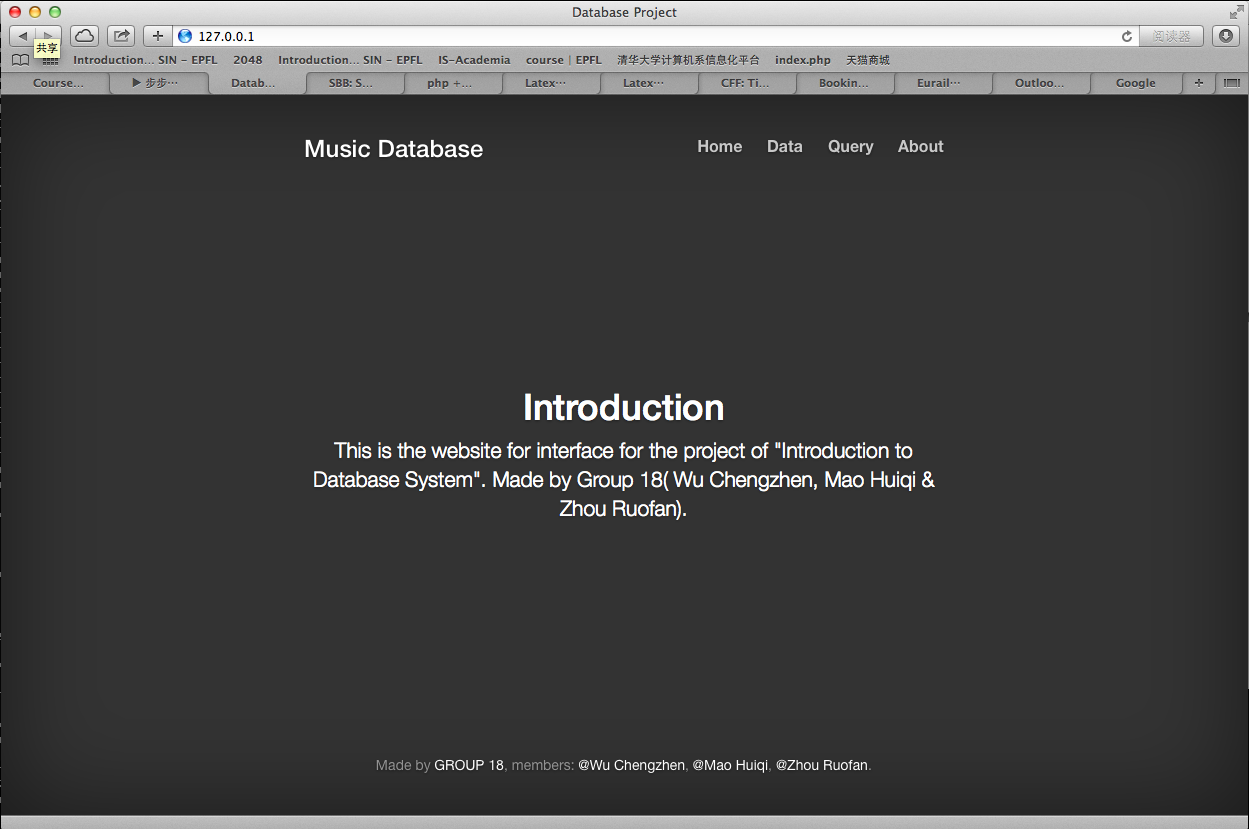
\includegraphics[width=14cm]{interface1}\\ \\
It's the index of our website. The website contains 4 parts: Home, Data, Query and About, and the functionally page is Data and Query.\\ \\
The screen shot of Data page is as below, the page shows the data of tables(you can select the table you want to see by clicking the link of table names, which are the yellow words on the uper part of the page). Each page would show 20 data and you can blowse more data by click the link of pages on the bottom part of the page. As the screen shot, it shows the 'artist' table. By moving your mouse onto those foreign keys, a prompt box showing the message of the table linked by the foreign key(as the screen shot, we move the mouse onto the 'areaid' and a box showing message of the name and type of the 'areaid').\\ \\
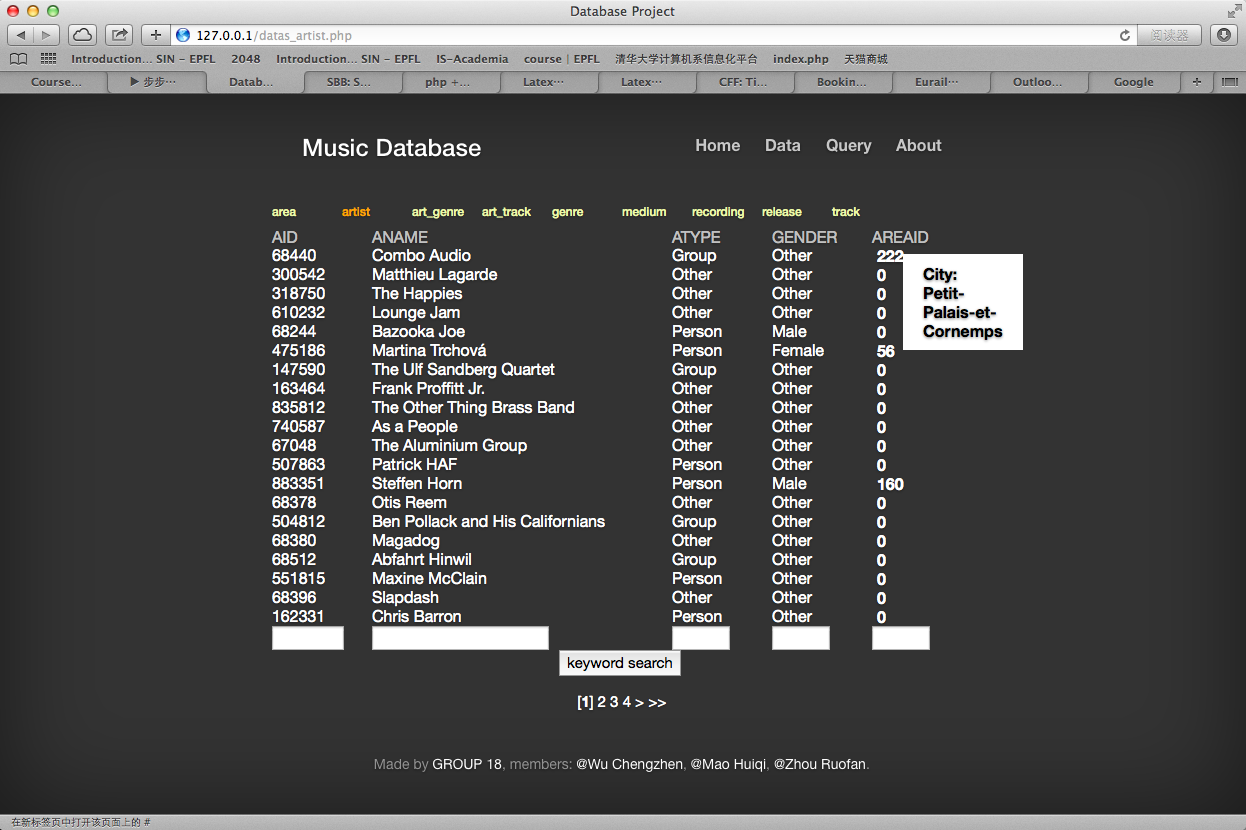
\includegraphics[width=13cm]{interface2}\\ \\
Under each row there's a input box, and you can use it to search for keyword. Just by clicking the "Keyword Search" you can filter the data of the table. For example, next screen shot shows the result as we input 'Person' under keyword 'atype' and 'male' under keyword 'gender'. \\ \\
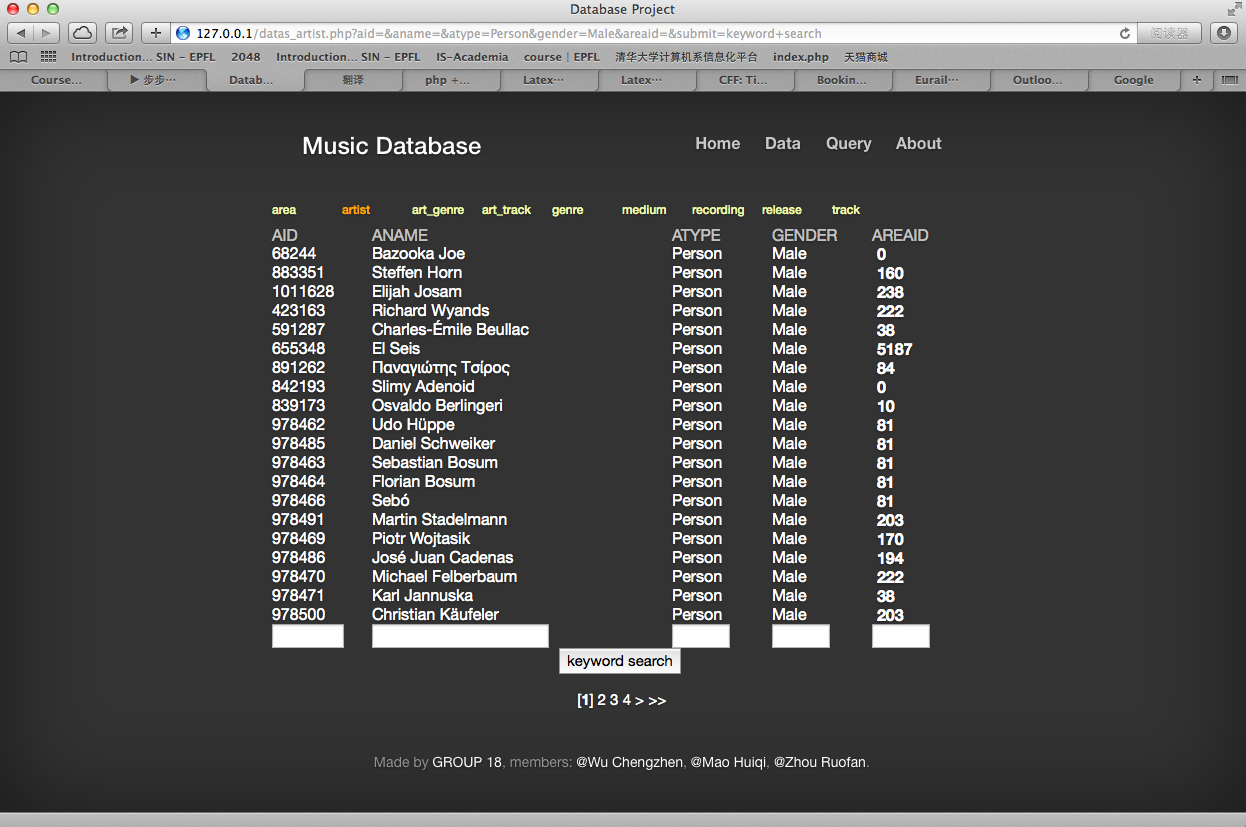
\includegraphics[width=13cm]{interface3}\\ \\
And we satisfied all the queries in the Query page, and you can see the results by clicking the query number.\\ \\
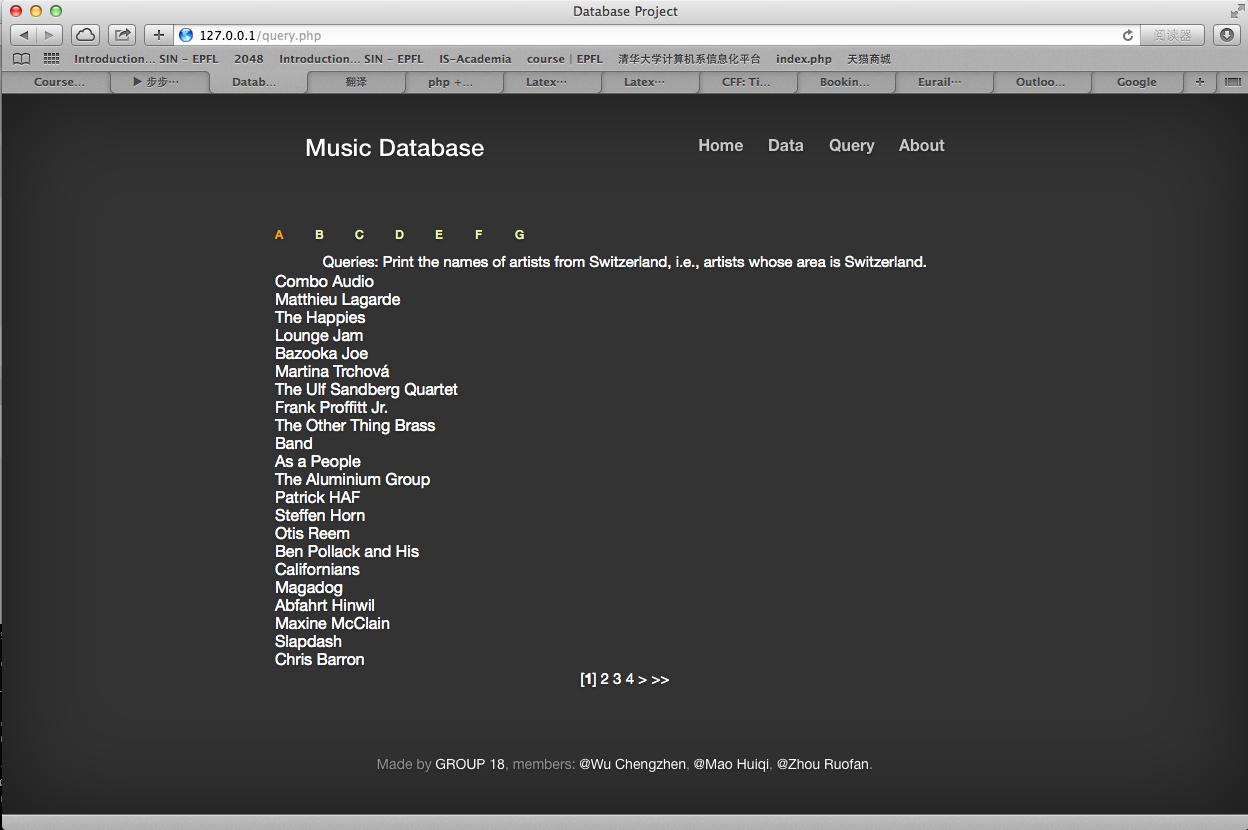
\includegraphics[width=13cm]{interface4}\\ \\
}

\end{document}
